\section{考察}
柔軟物の無い指では把持対象物C,Eが把持できなかった.把持対象物の形状に倣いによって摩擦力を大きくすることの不可能な柔軟で無い指では薄い板状の把持対象物Cでは接触面積が小さすぎるため把持できなかったと考えられる.把持対象物Eに関しても同様の理由で把持できなかったと考えられる.\par
ゲルを指先に取り付けた指は厚さが3mmと6mmの場合が全ての対象物が把持出来た.厚さが9mmの指では把持対象物Eの上部の突起部分をつまむことは出来た (\refig{gel_tumami}) が外周部の把持は出来なかった.この理由はゲルの厚さが9mmと比較的指が太くなってしまい指の開きが狭くなり指を把持対象物に接触できなかったからである.ゲルの厚さを厚くすると指の開きが狭くなるのでゲルの厚さは薄くするのが望ましいと考えられる.しかし,ゲルを薄くすると把持対象物に倣う接触面積が小さくなり把持力が低下が考えられる.本実験では最もゲルの厚さが薄い3mmの指での把持は安定していた.これよりゲルの厚さ3mmの時に把持力は低下しないと考えられる.よって3mmより薄く把持が安定する厚さの検証を今後の課題とする.\par
ゴムで覆ったスポンジを取り付けた指では,全ての厚さで把持対象物A,B,C,Dは把持出来,把持対象物Eは把持できなかった.把持対象物Eの上部をつまむ把持は全ての厚さの指で出来なかった.外周部の把持は厚みが8mm,10mmのときは指が太さにより外周部に指が沿わず把持が不可能であった.厚みが6mmのときは外周部に指を沿わすことは可能だが把持は不可能であった.この理由は把持力が不足していたためであると考えられる.把持力を大きくするためにスポンジを覆うゴムをより摩擦係数の大きなゴムに変更することが有効であると考えられる.\par
ばねを取り付けた指は全ての把持対象物を把持出来なかった.ばねの指が柔軟すぎる故に外側に反り返ってしまい把持対象物に倣うことが出来ず把持力が著しく不足しているためであると考えられる.本グリッパで用いたばねよりもより固いばねを使用すれば外側への反り返りが改善され把持が可能になると考えられる.

\begin{figure}[h]
 \begin{center}
  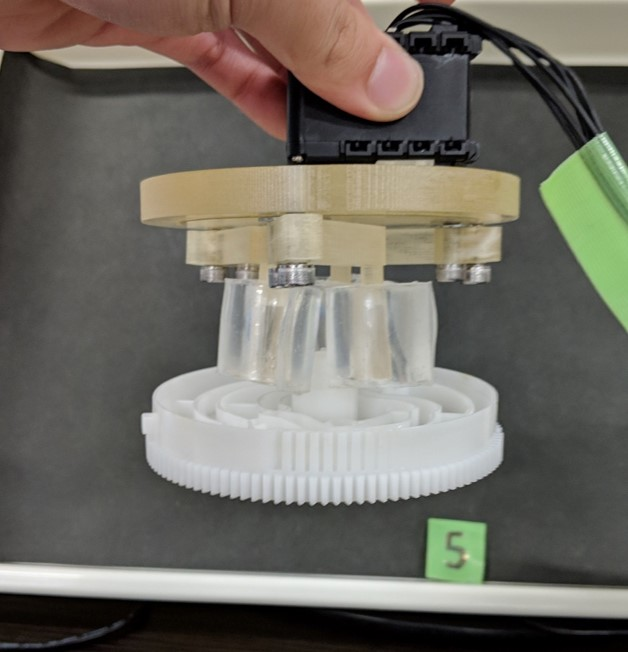
\includegraphics[scale=0.4]{../figure/gel_tumami.eps}
 \caption{厚さ9mmのゲルの指による把持対象物Eのつまみ把持}
  \label{fig::gel_tumami}
 \end{center}
\end{figure}


